\chapter{Cenni di Meccanica classica}
\label{meccanica_classica}
La Meccanica classica � una delle due branche maggiori della Meccanica, che si occupa di leggi che descrivono il moto di corpi sotto l'azione di un sistema di forze \cite{Wikipedia}.

\section*{Cinematica}
La Cinematica \cite{Douglas_classical_mechanics} � lo studio del moto di corpi materiali, senza considerare le cause e conseguenze di tale moto. La parte della Meccanica che si occupa delle cause e conseguenze del moto dei corpi � la Dinamica o Cinetica. La Cinematica fornisce una descrizione geometrica dei possibili moti.\\
Il soggetto mediante il quale vengono condotti gli studi in Cinematica � la particella, vale a dire un corpo immaginario, che occupa un singolo punto dello spazio. Un insieme di particelle le cui distanze relative rimangono invariate in ogni riferimento spaziotemporale. 

\subsection*{Moto rettilineo di una particella}

Data una particella in moto rettilineo uniforme (vedi figura \ref{fig:CinematicaLineare}), il suo moto pu� essere descritto secondo le seguenti quantit�:
\begin{description}
	\item[Posizione] Il vettore posizione della particella $P$ nel punto A
	
\begin{equation}
\begin{split}
\mathbf{r} & = (x_A,y_A,z_A) \quad \text{vettore posizione}\\
|\mathbf{r}| & = \sqrt{x_A^2 + y_A^2 + z_A^2}(m) \quad \text{magnitudine}
\end{split}
\label{eq:positionVector}
\end{equation}


	 

\item[Spostamento] Lo spostamento da $A$ a $B$ di $P$:

\begin{equation}
\begin{split}
\mathbf{r}_{AB} = \mathbf{r}_{B} - \mathbf{r}_{A} (m)
\end{split}
\label{eq:displacement}
\end{equation}


\item[Distanza] La distanza 

\begin{equation}
\begin{split}
\displaystyle s=\int_{t_1}^{t_2}{\sqrt{\Big(\dfrac{dx}{dt}\Big)^2 + \Big(\dfrac{dy}{dt}\Big)^2+ \Big(\dfrac{dz}{dt}\Big)^2}dt} (m)\\
\end{split}
\label{eq:distance}
\end{equation}
dove $t$ � il tempo.


\item[Velocit�] 

	\begin{itemize}
		\item media 
\begin{equation}
\begin{split}
\mathbf{\bar{v}} = \dfrac{\Delta \mathbf{r}}{\Delta t}(m/s)\quad \Delta t > 0
\end{split}
\label{eq:averageSpeed}
\end{equation}
				
		\item istantanea 

			\begin{equation}
				\begin{split}
					\mathbf{v} &= \displaystyle \lim_{\Delta t \rightarrow 0} \dfrac{\Delta \mathbf{r}}{\Delta t}\\
					|\mathbf{v}| &= \dfrac{ds}{dt}(m/s)\quad \text{magnitudine}
				\end{split}
			\label{eq:instantSpeed}
			\end{equation}
	
	\end{itemize}
	
\begin{figure}[h]
	\centering
		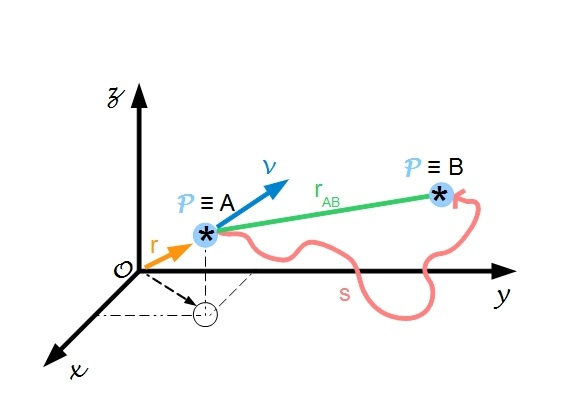
\includegraphics[width=.80\textwidth]{imgs/CinematicaLineare.jpg}
	\caption{Moto Rettilineo di una particella}
	\label{fig:CinematicaLineare}
\end{figure}
	
\item[Accelerazione]
	\begin{itemize}
		\item media 
			\begin{equation}
				\begin{split}
					\mathbf{\bar{a}} = \dfrac{\Delta \mathbf{v}}{\Delta t} \quad \Delta t > 0 (m/s^2)
				\end{split}
			\label{eq:instantSpeed}
			\end{equation}		
		\item istantanea 
			\begin{equation}
				\begin{split}
					\mathbf{a} = \displaystyle \lim_{\Delta t \rightarrow 0} \dfrac{\Delta \mathbf{v}}{\Delta t}(m/s^2) 
				\end{split}
			\label{eq:instantSpeed}
			\end{equation}
	\end{itemize}
\end{description}	

\section*{Moto Angolare di una particella}
Data una particella in moto circolare uniforme (vedi figura \ref{fig:CinematicaAngolare}), il suo moto pu� essere descritto secondo le seguenti quantit�:
\begin{description}
	\item[Posizione] Il vettore posizione della particella $P$ nel punto $A$ rispetto ad un asse di rotazione $O-z$ � $\mathbf{r}(t)$. La posizione angolare del punto $P$ �
			\begin{equation}
				\begin{split}
	  \mathbf{r}_{\perp}(t) = r_{\perp x} \cos \theta i + r_{\perp x} \sin \theta j (rad)
				\end{split}
			\label{eq:angularPositionVector}
			\end{equation}
	 


\item[Velocit�] 
La velocit� angolare � data da: 
		$\omega = \dfrac{d\theta}{dt}$ $(rad/s)$
	\begin{figure}[h]
	\centering
		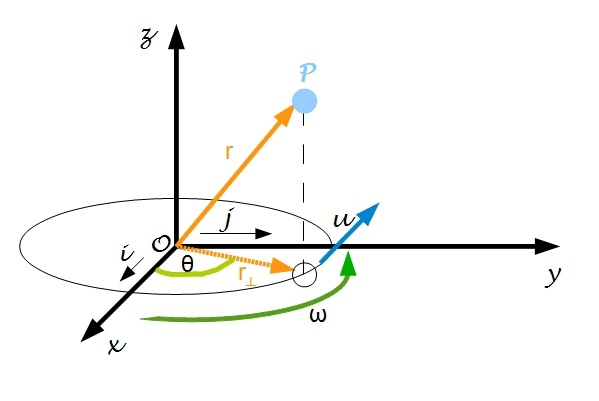
\includegraphics[width=.80\textwidth]{imgs/CinematicaAngolare.jpg}
	\caption{Moto Angolare di una particella}
	\label{fig:CinematicaAngolare}
\end{figure}
	
\item[Accelerazione]
L'accelerazione angolare � data da:
			\begin{equation}
				\begin{split}
					\alpha = \dfrac{d\omega}{dt}(rad/s^2)
				\end{split}
			\label{eq:acceleration}
			\end{equation}
\end{description}	
	
\section*{Dinamica (Cinetica)}
Branca della meccanica che si occupa di forze che producono, arrestano o modificano il moto di corpi. 
Le due leggi fondamentali della Dinamica sono quelle di Newton, in particolare la seconda �:
\begin{equation}
F = ma
\label{eq:secondoPrincipioNewton}
\end{equation}